% This must be in the first 5 lines to tell arXiv to use pdfLaTeX, which is strongly recommended.
\pdfoutput=1
% In particular, the hyperref package requires pdfLaTeX in order to break URLs across lines.

\documentclass[11pt]{article}

% Remove the "review" option to generate the final version.
\usepackage{ACL2023}
%\usepackage[review]{ACL2023}

% Standard package includes
\usepackage{times}
\usepackage{latexsym}
\usepackage{booktabs}
\usepackage{multirow} 
\usepackage{makecell}
\usepackage{graphicx}
\usepackage{listings}
\usepackage{tikz}
\usepackage{xcolor}
\usepackage{caption}

% Define custom colors
\definecolor{color1}{HTML}{1f77b4}
\definecolor{color2}{HTML}{ff7f0e}
\definecolor{color3}{HTML}{2ca02c}
\definecolor{color4}{HTML}{d62728}
\definecolor{color5}{HTML}{9467bd}
\definecolor{color6}{HTML}{8c564b}
\definecolor{color7}{HTML}{e377c2}
\definecolor{color8}{HTML}{7f7f7f}
\definecolor{color9}{HTML}{bcbd22}

% For proper rendering and hyphenation of words containing Latin characters (including in bib files)
\usepackage[T1]{fontenc}
% For Vietnamese characters
% \usepackage[T5]{fontenc}
% See https://www.latex-project.org/help/documentation/encguide.pdf for other character sets

% This assumes your files are encoded as UTF8
\usepackage[utf8]{inputenc}

% This is not strictly necessary, and may be commented out.
% However, it will improve the layout of the manuscript,
% and will typically save some space.
\usepackage{microtype}

% This is also not strictly necessary, and may be commented out.
% However, it will improve the aesthetics of text in
% the typewriter font.
\usepackage{inconsolata}
\usepackage{float}


% If the title and author information does not fit in the area allocated, uncomment the following
%
%\setlength\titlebox{<dim>}
%
% and set <dim> to something 5cm or larger.

\title{Team Cantharellus at SemEval-2025 Task 3: Hallucination Span Detection with Fine-Tuning on Weakly Supervised Synthetic Data}

% Author information can be set in various styles:
% For several authors from the same institution:
% \author{Author 1 \and ... \and Author n \\
%         Address line \\ ... \\ Address line}
% if the names do not fit well on one line use
%         Author 1 \\ {\bf Author 2} \\ ... \\ {\bf Author n} \\
% For authors from different institutions:
% \author{Author 1 \\ Address line \\  ... \\ Address line
%         \And  ... \And
%         Author n \\ Address line \\ ... \\ Address line}
% To start a seperate ``row'' of authors use \AND, as in
% \author{Author 1 \\ Address line \\  ... \\ Address line
%         \AND
%         Author 2 \\ Address line \\ ... \\ Address line \And
%         Author 3 \\ Address line \\ ... \\ Address line}

\author{Xinyuan Mo \and Nikolay Vorontsov \and Tiankai Zang \thanks{\hspace{0.6em}Equal contribution, authors are listed alphabetically.} \\
  %Department of Digital Humanities\\
  %Faculty of Arts \\
  University of Helsinki \\
  %Finland  \\
  \texttt{\{xinyuan.mo, nikolay.vorontsov, tiankai.zang\}@helsinki.fi} \\}

\begin{document}
\maketitle
\begin{abstract}
This paper describes our submission to SemEval-2025 Task-3: Mu-SHROOM, the Multilingual Shared-task on Hallucinations and Related Observable Overgeneration Mistakes, which mainly aims at detecting spans of LLM-generated text corresponding to hallucinations in multilingual and multi-model context. We explored an approach of fine-tuning pretrained language models available on Hugging Face. The results show that predictions made by a pretrained model fine-tuned on synthetic data achieve a relatively high degree of alignment with human-generated labels. We participated in 13 out of 14 available languages and reached an average ranking of 10th out of 41 participating teams, with our highest ranking reaching the top 5 place.


\end{abstract}


\section{Introduction}
Recent years have witnessed the rapid development of large language models (LLMs) and their applications in various fields of natural language processing \cite{wei2022chain, zhao2023survey}. However, content generated by LLMs occasionally contains inaccurate or fictitious information \cite{perkovic2024hallucinations}. The phenomenon in which natural language generation models often generate text that is nonsensical, or unfaithful to the provided source input is commonly referred to as “hallucinations” \cite{ji2023survey}. It is therefore a vital task to detect and identify hallucinated content so as to improve the reliability and trustworthiness of LLM-generated content.

SemEval 2025 Task 3 (Mu-SHROOM, the Multilingual Shared-task on Hallucinations and Related Observable Overgeneration Mistakes) \cite {vazquez-etal-2025-mu-shroom} proposes the task of detecting hallucination in content generated with LLMs. Different from the previous iteration, SemEval-2024 Task 6 \cite{mickus2024semeval}, in which the participants were asked to make binary decisions of whether a given context contains hallucination, the current task requires the participants to predict where the hallucinations occur. Specifically, the current task requires the participants to predict the spans of the hallucinated content within LLM outputs in 14 different languages.  

As is shown in the results of the previous iteration of this task \cite{mickus2024semeval}, it is effective to fine-tune pretrained language model for hallucination detection. We therefore further extended this approach from performing binary classification tasks to predict the spans of hallucinations. We explored fine-tuning a series of Transformer-based pretrained language models \cite{vaswani2017attention}, including text-to-text Transformer models \cite{raffel2020exploring} and BERT-based models \cite{devlin2018bert}, with training data created by ourselves. 

Building on this method, we developed the system based and participated in 13 out of 14 languages. In addition, we also applied the approach of named entity recognition (NER) as a baseline in order to provide a more comprehensive evaluation of our system's performance. We have released our code and other relevant material on GitHub \footnote{https://github.com/nicksnlp/Cantharellus.git}.


\section{Background}
Hallucination detection has been an extensively researched topic in recent years. One promising solution for hallucination detection is to utilize the self-evaluation ability of LLMs to judge the factual correctness of a given statement, leveraging the fact that LLMs have possessed a rich knowledge base \cite{li2024dawn, zhang2024self}. Many existing studies focus on the binary classification of hallucination. For instance, SelfCheckGPT \cite{manakul2023selfcheckgpt} is built on the idea that when an LLM is familiar with a particular concept, the responses it generates are likely to be consistent and contain similar facts. In the HaluEval 2.0 benchmark \cite{li2024dawn}, the hallucination detection approach is built by first extracting factual statements from LLM responses, then determining the trustfulness of these statements with respect to world knowledge by taking advantage of the vast knowledge base of LLMs. Similarly, MIND \cite{su2024unsupervised} introduces a similar approach that leverages the internal states of LLMs for real-time hallucination detection without requiring manual annotations. GraphEval \cite{sansford2024grapheval} proposes a method of detecting inconsistencies with respect to provided knowledge using a knowledge-graph approach.

Prompt engineering is a crucial technique for extending the capabilities of LLMs \cite{sahoo2024systematic}. A commonly used strategy is few-shot prompting, which refers to the technique of constructing prompts using a small set of demonstrative input-output examples \cite{lazaridou2022internet, ma2023fairness}. Another method that has been proved effective is chain-of-thought (CoT) prompting, which is achieved by guiding the LLM to think step by step to perform complex reasoning tasks \cite{wei2022chain, zhang2022automatic, chen2023you}.

Named entity recognition (NER) \cite{yadav2019survey} is the task of identifying named entities such as person, location and organization in text,  which are often central to factual inconsistencies in LLM-generated text. Deep learning approaches have increasingly been adopted for NER and have exhibited impressive abilities across various domains and languages \cite{li2020survey, song2021deep, liu2022chinese}. Recent research also explores the possibility of integrating prompting techniques into NER tasks by utilizing LLMs \cite{shen2023promptner, hu2024improving}. While NER is limited to identifying predefined entity types and cannot assess the broader context or relationships between entities, it can still serve as a tool for detecting potential sources of hallucinations, making it a possible referential benchmark.

\section{System Overview}

\subsection{Fine-tuning Procedure}
The goal of this task is to detect hallucinations and identify their spans, defined by character indices, within an answer generated in response to a question. One of the ways to address this is to reformulate the problem as a token classification task, where hallucinated tokens are labeled as 1 and non-hallucinated tokens as 0.

We conducted experiments on Transformer-based models to evaluate their performance on this task. Given the limited size of the validation sets (50 labeled data points per language), all base models were trained on our self-generated data (approximately 2K data points per language).

\subsubsection{Data Construction}
It is crucial to have sufficient data to fine-tune the pretrained language models in order to enhance their performance on specific tasks. However, the training sets provided by the organizers are unlabeled and are thus unable to be used directly for fine-tuning. Therefore, we proposed a semi-automatic approach to construct labeled data by prompting state-of-the-art generative language models, specifically GPT-4o.

In order to obtain the data in a manner similar to that of the labeled validation sets provided by the organizers, we explored a combination of few-shot prompting and chain-of-thought (CoT) prompting techniques. Specifically, we utilized several data points in the labeled validation set as learning examples and guided the LLM to infer hallucinated content based on the spans marked by human annotators in those samples. 

A closer examination of the generation revealed that the LLM often misidentified the span boundaries of the hallucinated words it generated. Therefore, we optimized the pipeline of data construction by prompting the LLM to identify the hallucinated words first and subsequently convert the tokens to spans. To that end a simple algorithm was applied, which would automatically iterate through the model output text, locate each hallucinated word, and mark its start and end character indices. This additional step significantly increases the quality of generated annotations. 

A number of 2,371 data points in English was constructed initially for testing purposes. In addition to those, ultimately, we constructed 2000 data points for each of the 12 other languages in which we participated. The detailed prompt is shown in Appendix~\ref{sec:prompts}.


\subsubsection{Base Models and Token Classification Setup}
For fine-tuning, we experimented with a diverse set of pretrained Transformer-based models \cite{vaswani2017attention}, starting with monolingual architectures and later transitioning to multilingual models, which support all 13 target languages, to achieve broader language coverage. We focused on the English monolingual models to compare their performance with that of the multilingual models. Table \ref{tab:monolingual_models} and Table \ref{tab:multilingual_models} in the Appendix~\ref{sec:appendix} show the details of the base models.

\texttt{AutoModelForTokenClassification} classes from the Hugging Face \texttt{transformers} library \cite{wolf-etal-2020-transformers} are used to load each of the base models and their tokenizers. This step attaches a randomly initialized linear classification layer on top of the Transformer encoder, ensuring the model outputs token-wise predictions for binary classes (1 or 0 for hallucination or non-hallucination, respectively). The label mappings are explicitly defined through the model's configuration using \texttt{id2label} and \texttt{label2id}. The model performs sequence labeling, where each token in the input sequence is assigned a binary label based on both its own identity and its contextual information from the entire sequence.






\subsection{Performance Evaluation}
 A system's capability to capture hallucination spans is assessed along two main dimensions: (i) the overlap between the system’s predicted hallucination spans and human annotations, and (ii) the alignment in reasoning between the system and human annotators, reflected in the correlation between the confidence of system predictions and the agreement of human annotators on hallucination spans.

These two evaluation dimensions were measured using Intersection over Union (IoU) and Correlation (Cor) scores, respectively. 

The IoU score quantifies the overlap between predicted hard labels and reference hallucination spans by dividing the size of their intersection by the size of their union. If neither the prediction nor the reference contains hallucinations, the score is set to 1.0.

The Cor score quantifies the agreement between predicted soft labels and reference confidence levels, which are computed as the fraction of annotators who labeled a span as hallucinated. This agreement is measured using Spearman’s rank correlation \cite{spearman1987proof}. The score ranges from -1 to 1, where 1 indicates perfect agreement, 0 signifies no correlation, and -1 represents complete disagreement.



\section{Experimental Setup}

\subsection{Model Fine-Tuning}
The fine-tuning procedure began with pre-processing the training data, aligning tokens with binary labels to indicate hallucination. Fine-tuning Stage 1 was conducted using our auto-generated training data. This step is followed by fine-tuning Stage 2 using the labeled validation sets provided by the task's organizers, either with all available sets (for multilingual models) or the validation set corresponding to the specific test language (for both monolingual and multilingual models).
Model performance was assessed for both fine-tuning stages. The experimental architecture is illustrated in Figure~\ref{fig:fine_tuning_pipeline}.


\begin{figure*}[ht]
    \centering    
    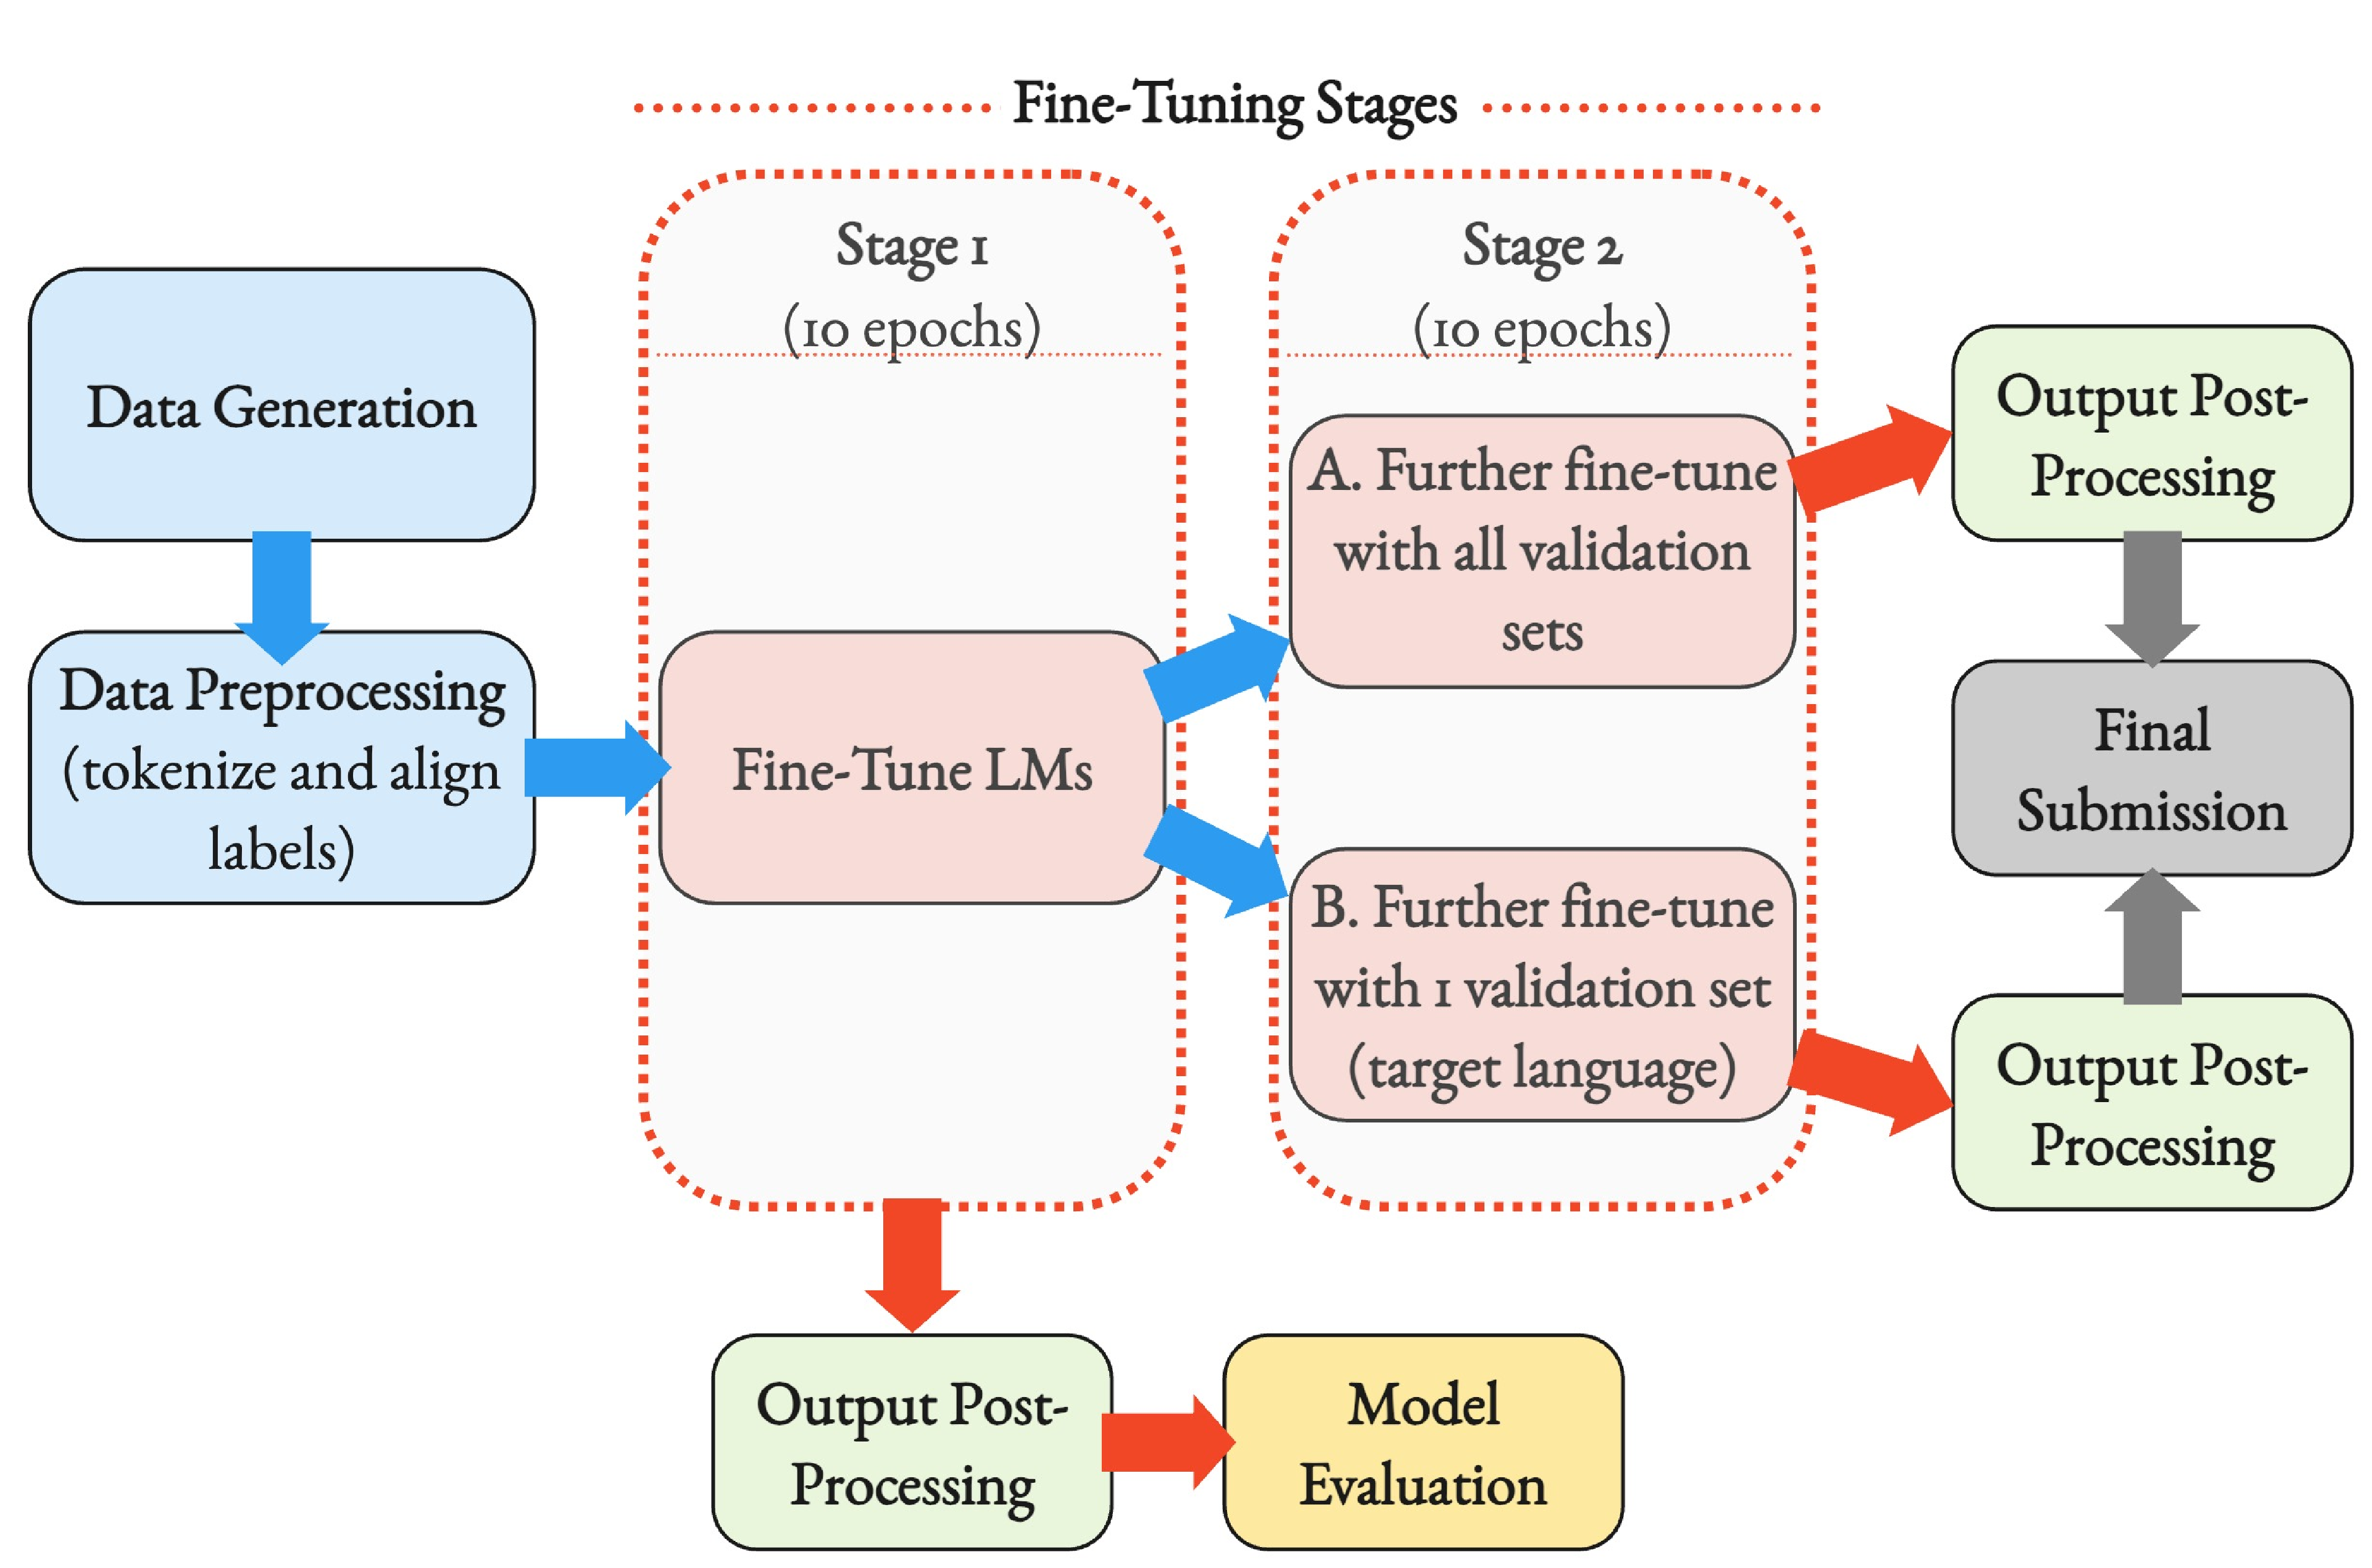
\includegraphics[width=0.7\textwidth]{images/pipeline.pdf}
    \caption{Fine-Tuning Pipeline.}
    \label{fig:fine_tuning_pipeline}
    \vspace{-1em}
\end{figure*}

\subsubsection{Data Preprocessing}
\textbf{Label Alignment}  
\label{sec:Label-Alignment}
In all labeled datasets used for fine-tuning, hallucination spans are provided in the format \texttt{[start\_index, end\_index]}. We leveraged this span information to automatically generate labels for each token before feeding the training data into the base models. After tokenization, labels are assigned based on each token’s \texttt{offset\_mapping}: tokens whose start and end indices fall within any hallucination span receive a label of 1, while all others are labeled 0.

\textbf{Data Split}  
We used a 9:1 training-validation split on our self-generated labeled data, resulting in approximately 1,800 training samples and 200 validation samples for each of the 13 languages. These included nine announced target languages: Arabic, German, English, Spanish, Finnish, French, Hindi, Italian, and Chinese, as well as four surprise languages: Czech, Catalan, Basque and Farsi, which were revealed only after the test set was released by the organizers.

We evaluated our models' performance using the labeled validation sets provided by the organizers after fine-tuning. We chose these sets as test data due to (i) their high-quality hallucination spans annotated by human annotators and (ii) their likely similarity to the data used by the organizers for final evaluation. In contrast, our semi-automatically generated labeled data were not reviewed by native speakers and may be of lower quality. However, since labeled validation sets were not available for the four surprise languages, we generated 50 labeled data points for each of these languages for testing purpose using the same method as for our training data.


\subsubsection{Hyperparameters for Tokenization and Training}
For the fine-tuning procedure, the same set of hyperparameters for both tokenization and training was applied to all base models. The same hyperparameters were applied to both fine-tuning Stage 1 and Stage 2.

\textbf{Tokenizer Parameters}  
Only the generated answers (\texttt{model\_output\_text}) were tokenized as input for model fine-tuning, while the inquiries (\texttt{model\_input}) were not used. Tokenization included \texttt{padding} with a maximum length of \texttt{128} tokens and the application of \texttt{truncation}. Additionally, \texttt{return\_offsets\_mapping} was set to \texttt{True}, as the offset mapping is crucial for converting hallucination spans into token-level labels after tokenization. Details on this process are discussed in Section~\ref{sec:Label-Alignment}.


\textbf{Training Parameters}
The training process was configured with a predefined set of parameters. The learning rate was set to 2e-5. Batch sizes were defined as 8 for both training and evaluation (\texttt{per\_device\_train\_batch\_size = 8} and \texttt{per\_device\_eval\_batch\_size = 8}). The number of training epochs was set to 10, as our preliminary experiments indicated that model performance plateaued around this point. Additionally, a \texttt{weight\_decay} of 0.01 was applied to the training arguments.


\subsubsection{Output Post-Processing}
During the inference stage, the input text was tokenized and processed by the models to obtain logits for each token to be assigned to one of the two possible labels. The logits were later converted to probabilities using the softmax function, which normalized the scores along the label dimension:

\[
P(y_i \mid x) = \frac{\exp(z_i)}{\sum_{j} \exp(z_j)}
\]

In the formula above, $P(y_i \mid x)$ represents the probability of the $i$-th label for a given token, and $z_i$ the corresponding logit.

To identify hallucination spans, contiguous tokens labeled as "1" (hallucinated) were grouped based on their start and end indices derived from the token offset mappings. Adjacent "1" labels with consecutive indices were treated as a single span. For each span, the average probability of the "1" labels was computed, providing a confidence score that reflects the model's uncertainty regarding the span's validity. This average probability, along with the start and end indices of each hallucination span, together form the soft labels. Hard labels are then derived by selecting spans from the soft labels with a probability of 0.5 or higher.
   
\subsection{Benchmarks for Evaluation}
To assess whether fine-tuning improves model performance in hallucination detection, we evaluate the predictions of the models from fine-tuning Stage 1 on the organizers' validation sets. This evaluation uses Cor and IoU scores and compares the results against three benchmarks: (i) the benchmark provided by the organizers and (ii) the performance of a pretrained multilingual Named Entity Recognition (NER) model. 

\textbf{Organizers' Benchmark}
The benchmark provided by the organizers was derived by fine-tuning the multilingual model \texttt{FacebookAI/xlm-roberta-base} \cite{DBLP:journals/corr/abs-1911-02116} using the labeled validation sets they released. These validation sets contained 50 data points per language across 10 languages, excluding the four surprise languages.

Cor and IoU scores were computed for each test language. The base model was trained on validation sets from all languages except the test language, ensuring no test data leakage. This process was repeated for each language, yielding 10 fine-tuned models, each tailored to a specific test language. Fine-tuning was performed using the \texttt{model\_output\_text} and two label types, which classified tokens as either hallucinated or non-hallucinated.



\textbf{NER Benchmark}
A close examination of the sample set shows that a considerable number of hallucinations involve proper nouns, such as names of people, places or organizations. We therefore proposed using a model fine-tuned for NER to make predictions without further fine-tuning, in order to serve as a comparison to the models fine-tuned specifically for this task.

This benchmark was created using the pretrained NER model \texttt{51la5/roberta-large-NER} \cite{conneau2019unsupervised}, a large multilingual language model supporting all 13 of our target languages. Trained on 2.5TB of filtered CommonCrawl data, this model is an XLM-RoBERTa-large variant fine-tuned on the CoNLL-2003 dataset for English NER. We used the model as-is, without any additional fine-tuning. As a result, it treated all named entities as hallucinations.

\section{Results}
Our submission included 21 models in total, with different combinations of models and training data used. These were the following:
\begin{itemize}
    \item Multilingual models trained on the synthetic data only (26.3K data points, 10 epochs)
    \item Multilingual models trained on the synthetic data (26.3K data points, 10 epochs) and fine-tuned further with a single validation set for the target language (50 data points, 10 epochs)
    \item Multilingual models trained on the synthetic data (26.3K data points, 10 epochs) and fine-tuned further with all the validation sets (650 data points, 10 epochs)
    \item English language models trained on the synthetic data only (2.3K data points, 10 epochs)
    \item English language models trained on the synthetic data only (2.3K data points, 10 epochs) and fine-tuned further with a single validation set for the English language (50 data points, 10 epochs)
\end{itemize}

From all the combinations the models trained on the maximum amount of data showed superior results, with some minor exceptions (see Appendix~\ref{sec:iou_scores}). Our best average performing model was based on \texttt{xlm-roberta-large}.

As opposed to the initial submission, when the models were trained on the generated answers only (\texttt{model\_output\_text}), we have conducted an additional test, and trained \texttt{xlm-roberta-large} base model again with the same parameters, but using a concatenation of the questions and the answers as the training input, separating them with an additional special token \texttt{'<@@>'}. We have used similar joint input for inference and adjusted the spans accordingly. The results of such training have outperformed all of our other approaches, with a significant increase of scores for all of the languages except English and Chinese. A comparative summary of the models' IoU scores is shown in Appendix~\ref{sec:iou_scores_appendix}.

\section{Conclusion and Limitations}
As our participation in SemEval-2025 Task-3, we proposed the approach of fine-tuning language models with synthetic data for hallucination span prediction. The results demonstrate that our system achieved competitive scores across various languages. Our approach is proved effective as the scores rank as high as 5th in certain languages.

The fact that the model is exclusively fine-tuned on data constructed by LLM suggests that this approach is a feasible and effective strategy for the task of hallucination span prediction, particularly under the circumstance where human-labeled training data is absent. However, it is worth pointing out that LLM-based synthetic data are potentially more heavily subject to limitations compared with hand-crafted data. A closer examination suggests that the quality of the synthetic data does not match that of the validation and test sets provided by the organizers. Across various languages, the synthetic data can often be shorter or significantly longer in output length, cover a narrower range of topics, and propose less sophisticated question-and-answer pairs than those in the validation and test sets. These problems can supposedly be addressed through few-shot prompting and more elaborate prompt-engineering. It is also important to mention, that although various efforts have been made in both prompting and post-processing to increase the likelihood that the spans correctly indicate the hallucinated texts, the final output is still prone to errors and may not match the accuracy of human-annotated data, although it was reported that models trained on data generated in a similar manner outperform models trained on real-world data in certain tasks \cite{li-etal-2023-synthetic}. In addition, it should also be noted that predominantly only one model, GPT-4o, is used for data synthesis. This lack of variation in model choice may limit the diversity of the synthetic data, which could in turn potentially reinforce the intrinsic biases of the model in question.

Future directions could include creating and utilizing training data in large quantities, as well as optimizing prompting techniques to obtain higher-quality training data from LLMs. Another viable approach would be to adopt more advanced state-of-the-art models for either data creation or fine-tuning.

\section{Acknowledgments}
We would like to express our gratitude to our supervisor, Jörg Tiedemann, for valuable suggestions and guidance throughout this work.

\section{Individual Contributions}
\textbf{Xinyuan Mo: } Model fine-tuning, including I. constructing python script for: 1) data preprocessing (tokenizing and aligning labels), 2) fine-tuning multiple base models, and 3) output generation and scoring (integrating code "\texttt{scorer.py}" from the organizers to generate scores), and II. executing the fine-tuning and scoring procedure on Puhti supercomputer. 

Paper writing of the sections: System Overview (excluding the "Data Construction" subsection) and Experimental Setup.
\\

\textbf{Nikolay Vorontsov: } Experimenting with various options for data construction, including: 1. direct prompting with Gemini and GPT through APIs and output post-processing; 2. generating questions-answers pairs from given input texts (with AutoModelForQuestionAnswering, QuestionAnsweringPipeline) and refining with a generative model. 3. converting labelled datasets into translated versions preserving labelling (with google translator API) and output post-processing.

Development of the system for labelling the datasets with LLMs through API (used as another baseline during development), automated post-processing of the output, union and intersections of the models' predictions.

Development of alternative fine-tuning strategies with different training parameters, including LoRA parameter-efficient fine-tuning of Llama 7B model with 4-bit quantization. Alternating tokenization pre-processing and post-processing to include both questions and answers during training and inference stages of models. Setting up an environment on Puhti supercomputer, running training and prediction jobs. 

Limited project management including setting up shared repositories, communication channels, submission of the final predictions to the shared task.

Paper writing of the Results section, analysis of the results, creation of figures and formatting.
\\

\textbf{Tiankai Zang: } Data construction, including 1) designing and testing various prompting techniques for optimal outputs, 2) overseeing the data generation process and making adjustments as needed, and 3) converting the data to desired format for fine-tuning. 

Paper writing of the sections: Abstract, Introduction, Background, System Overview ("Data Construction" subsection), Conclusion and Limitations.

\bibliography{custom}
\bibliographystyle{acl_natbib}


\newpage

\appendix
\clearpage

\onecolumn
\section{IoU Scores for models trained on synthetic data and fine-tuned further with either: (1) all the validation sets (multilingual models); (2) single validation set (English language models)}
\label{sec:iou_scores_appendix}

    \centering
    
\includegraphics[width=0.8\textwidth]{images/plot.pdf}
    %\caption{IoU Scores for models trained on synthetic data and fine-tuned further with either: (1) all the validation sets (multilingual models); (2) single validation set (English language models).}
    %\label{fig:iou_scores}

\section{Base Models Used}
\label{sec:appendix}
\begin{table}[h]
    \centering
    \captionsetup{justification=centering, singlelinecheck=false}    \renewcommand{\arraystretch}{1.5}  % Increase row height
    \begin{tabular}{|l|p{8.5cm}|}
        \hline
        \textbf{Model} & \textbf{Description} \\ \hline\hline
        \texttt{google-bert/bert-base-cased}   &  109M parameters, pretrained for masked language modeling (MLM) \cite{DBLP:journals/corr/abs-1810-04805}. \\ 
        \hline
        \texttt{deepset/roberta-base-squad2}   & 124M parameters, a RoBERTa-base model fine-tuned for extractive question answering \cite{deepset_roberta_squad2}. \\ 
        \hline
        \texttt{microsoft/deberta-v3-base}  & 86M backbone parameters, pretrained for replaced token detection \cite{he2021debertav3}. \\ 
        \hline
    \end{tabular}
    \caption{Monolingual (English) base models for fine-tuning}
    \label{tab:monolingual_models}
\end{table}

\begin{table}[h]
    \centering    
    \captionsetup{justification=centering, singlelinecheck=false}    \renewcommand{\arraystretch}{1.5}  % Increase row height
       \begin{tabular}{|l|p{8.5cm}|}
        \hline
        \textbf{Model} & \textbf{Description} \\ \hline\hline
        \multicolumn{1}{|p{5.3cm}|}{\parbox[t]{6cm}{\texttt{google-bert/bert-base-\\multilingual-cased}}} & 179M parameters, 104 languages, pretrained for MLM and next sentence prediction (NSP) \cite{DBLP:journals/corr/abs-1810-04805} \\ \hline
        \multirow{2}{*}{\parbox[t]{6cm}{\texttt{google/umt5-small} \\ \texttt{google/umt5-base}}} & \multirow{2}{8.5cm}{179M parameters, 102 languages \cite{chung2023unimax}}\\ \cline{1-1}
        & \\ \hline
        \multirow{2}{*}{\parbox[t]{6cm}{\texttt{FacebookAI/xlm-roberta-base} \\ \texttt{FacebookAI/xlm-roberta-large}}} & \multirow{2}{8.5cm}{279M (base) / 561M (large) parameters, 94 languages, pretrained for MLM \cite{DBLP:journals/corr/abs-1911-02116}}\\ \cline{1-1}
        & \\ \hline
    \end{tabular}
    \caption{Multilingual base models for fine-tuning}
    \label{tab:multilingual_models}
\end{table}

\twocolumn
\clearpage
\raggedright
\section{Prompt for Data Construction}
\label{sec:prompts}
\small
\ttfamily
""Given information 1:\\
\hspace*{1em} "model\_input": "How many genera does the Erysiphales order contain?",\\
\hspace*{1em} "model\_output\_text": "The Elysiphale order contains 5 genera.",\\
\hspace*{1em} "Model\_output\_text" is supposed to be the answer to the question in "model\_input" but contains some errors (hallucinations) which contradict the fact. Your task is to specify the spans of the erroneous texts and mark them as "soft\_labels".\\
\hspace*{1em} In order to do this, firstly, you should locate the erroneous texts based on the question asked in "model\_input" as well as the fact. For example, in this case, Elysiphale order contains 4 genera instead of 5; the span of "4" is [31, 32]; and it has a probability of 1 to be erroneous. Therefore, you should specify this in the following way:\\
\hspace*{2em} \{ "start": 30, "prob": 1, "end": 31 \}.\\
\hspace*{1em} Apply the same approach to other parts of the text. The final result is:\\
\hspace*{2em} "soft\_labels": [\\
\hspace*{3em} \{ "start": 4, "prob": 0.2, "end": 14 \},\\
\hspace*{3em} \{ "start": 30, "prob": 1, "end": 31 \},\\
\hspace*{3em} \{ "start": 31, "prob": 0.2, "end": 38 \}],\\
\hspace*{2em} "hard\_labels": [[30, 31]],\\
For your information, here are two more examples:\\
Example 1\\
\hspace*{1em} "model\_input": "Do all arthropods have antennae?",\\
\hspace*{1em} "model\_output\_text": "Yes, all insects and arachnids (including spiders, scorpions, and ticks) have at least one antenna.",\\
\hspace*{1em} "soft\_labels": [\\
\hspace*{2em} \{ "start": 10, "prob": 0.2, "end": 12 \},\\
\hspace*{2em} \{ "start": 12, "prob": 0.3, "end": 13 \},\\
\hspace*{2em} \{ "start": 13, "prob": 0.2, "end": 18 \},\\
\hspace*{2em} \{ "start": 25, "prob": 0.9, "end": 31 \},\\
\hspace*{2em} \{ "start": 31, "prob": 0.1, "end": 37 \},\\
\hspace*{2em} \{ "start": 45, "prob": 1, "end": 49 \},\\
\hspace*{2em} \{ "start": 49, "prob": 0.3, "end": 65 \},\\
\hspace*{2em} \{ "start": 65, "prob": 0.2, "end": 69 \},\\
\hspace*{2em} \{ "start": 69, "prob": 0.9, "end": 83 \}],\\
Example 2\\
\hspace*{1em} "model\_input": "What did Petra van Staveren win a gold medal for?",\\
\hspace*{1em} "model\_output\_text": "Petra van Stoveren won a silver medal in the 2008 Summer Olympics in Beijing, China.",\\
\hspace*{1em} "soft\_labels": [\\
\hspace*{2em} \{ "start": 10, "prob": 0.2, "end": 12 \},\\
\hspace*{2em} \{ "start": 12, "prob": 0.3, "end": 13 \},\\
\hspace*{2em} \{ "start": 13, "prob": 0.2, "end": 18 \},\\
\hspace*{2em} \{ "start": 25, "prob": 0.9, "end": 31 \},\\
\hspace*{2em} \{ "start": 31, "prob": 0.1, "end": 37 \},\\
\hspace*{2em} \{ "start": 45, "prob": 1, "end": 49 \},\\
\hspace*{2em} \{ "start": 49, "prob": 0.3, "end": 65 \},\\
\hspace*{2em} \{ "start": 65, "prob": 0.2, "end": 69 \},\\
\hspace*{2em} \{ "start": 69, "prob": 0.9, "end": 83 \}],\\
\hspace*{1em} "hard\_labels": [ [25, 31], [45, 49], [69, 83] ],\\
You should:\\
1. Study the examples above, understand why and how certain texts in "model\_output\_text" are labeled.\\
2. Please generate a similar example, in which you ask a question, answer it with one or a few hallucinations deliberately, and label the hallucinated words (instead of the spans and probabilities of possible hallucinations).\\
3. You are encouraged to include more than two hallucinated words in your output.\\
4. You do not need to explain your annotations.\\
5. The output format should be JSON.\\
The format should be:\\
\hspace*{1em} "model\_input":\\
\hspace*{1em} "model\_output\_text":\\
\hspace*{1em} "hallucinated\_words": <list all hallucinated words in "model\_output\_text" here>\\
\noindent
generate your response in \{lang\}""

\rmfamily
\normalsize % Restore normal font size


The above prompt was used as an input for dialogue systems, with a language specified inside \texttt{\{lang\}}. The output was then manually copied and pasted into a .jsonl file, repetitive outputs were eliminated. Hard labels were created by running the following example code:

\lstset{
    language=Python,
    basicstyle=\ttfamily\scriptsize,
    keywordstyle=\color{blue},
    commentstyle=\color{gray},
    stringstyle=\color{red},
    breaklines=true,
    frame=single
}



\begin{lstlisting}
import json

current_id = 1  

with open('eu-sim-val-raw.json', 'r', encoding='utf-8') as file:
    data = json.load(file)

with open('eu-sim-val.jsonl', 'a', encoding='utf-8') as output_file:

    for entry in data:
        model_input = entry["model_input"]
        model_output_text = entry["model_output_text"]
        spans = []

        for word in entry["hallucinated_words"]:
            start_index = 0
            while True:
                start_index = model_output_text.find(word, start_index)  
                if start_index == -1:
                    break
                end_index = start_index + len(word)
                spans.append([start_index, end_index])
                start_index = end_index 

        result = {
            "id": current_id, 
            "created_with": "GPT4o",
            "lang": "eu",  
            "model_input": model_input,
            "model_output_text": model_output_text,
            "hard_labels": [[start_index, end_index] for start_index, end_index in spans]
        }

        current_id += 1

        json.dump(result, output_file, ensure_ascii=False)
        output_file.write("\n")
\end{lstlisting}
\newpage
\onecolumn
\clearpage

\newpage
\onecolumn
\section{IoU Scores for Different Fine-Tuning Strategies and Models}
\label{sec:iou_scores}

    \centering
    
\includegraphics[width=0.9\textwidth]{images/xlm-roberta-large-10ep-M_with_separator.txt.pdf}
    \label{fig:xlm-roberta-large-10ep-M_with_separator}
    \centering
    
\includegraphics[width=0.9\textwidth]{images/xlm-roberta-large-10ep-M.txt.pdf}
    \label{fig:xlm-roberta-large-10ep-M}

    \centering
    
\includegraphics[width=0.9\textwidth]{images/xlm-roberta-base.txt.pdf}
    \label{fig:xlm-roberta-base}

    \centering
    
\includegraphics[width=0.9\textwidth]{images/umt5-small-10ep-M.txt.pdf}
    \label{fig:umt5-small-10ep-M}

    \centering
    
\includegraphics[width=0.9\textwidth]{images/umt5-base-10ep-M.txt.pdf}
    \label{fig:umt5-base-10ep-M}

    \centering
    
\includegraphics[width=0.9\textwidth]{images/bert-base-multilingual-cased.txt.pdf}
    \label{fig:bert-base-multilingual-cased}

\twocolumn

\end{document}
